\section{Round-Wire Analysis and Two-Dimensional Calibration}
\label{chapter:03}

% block-id: 03.round_derivation.heading
\hypertarget{03.round_derivation.heading}{}
\subsection{Round-wire radial equation and normalization}

% block-id: 03.round_derivation.p1
\hypertarget{03.round_derivation.p1}{}
Axial current inside a long straight round wire satisfies (1/r)d(r dJz/dr)/dr=κ²Jz. Finiteness at the axis selects I\(_0\)(κr), and the total complex-current constraint together with \(\int\)\(_0\)\(^a\)rI\(_0\)(κr)dr=aI\(_1\)(κa)/κ fixes its coefficient. Surface axial electric field divided by total current gives internal impedance per unit length. An independent Joule integral of current density checks the relationship between its real part and loss. The derivation uses the same RMS phasors as the main text.

% block-id: 03.analytic.heading
\hypertarget{03.analytic.heading}{}
\subsection{Round-wire internal-field calibration}

% block-id: 03.analytic.p1
\hypertarget{03.analytic.p1}{}
The radial current and internal impedance of a long straight round wire follow \eqref{eq:E03}. At 200 kHz, the skin depth δ=\metric{skin_depth} mm is approximately 0.148 times the radius, and current concentrates near the surface. DC resistance is \metric{q1_rdc} mΩ/m, AC resistance is \metric{q1_rac} mΩ/m, and Rac/Rdc=3.64720, giving a loss of \metric{q1_loss} W/m. The radial profiles and cross-sectional magnitude appear in Fig.~\ref{fig:q1_profile} and Fig.~\ref{fig:q1_cross_section}. Radial phase is continuously unwrapped, showing the amplitude attenuation and phase change associated with skin diffusion. The analytical impedance concerns the conductor's internal field.

% block-id: 03.analytic.p2
\hypertarget{03.analytic.p2}{}
Independent two-dimensional disk diffusion uses three meshes with 353, 1389, and 5573 nodes, normalized by total complex current. With refinement, relative Rac error against analysis decreases from 7.05×10⁻³ to 2.30×10⁻⁴ and finally 1.79×10⁻⁶. The finest-grid relative power-integral difference is 3.07×10⁻⁶, as shown in Fig.~\ref{fig:q1_fem_error}. These results verify discretization, normalization, and power postprocessing for the isolated round-wire internal-field problem. The cross-sectional illustration uses linear interpolation of analytical radial samples and an axisymmetric mapping; subsequent multistrand models use their actual conductor field solutions.

% block-id: 03.equation.E03
\hypertarget{03.equation.E03}{}
\hypertarget{E03}{}
\begin{equation}
\begin{gathered}
\delta=(\pi f\mu\sigma)^{-1/2} \\
\kappa=(1+j)/\delta \\
J_z(r)=\frac{I_t\kappa I_0(\kappa r)}{2\pi a I_1(\kappa a)} \\
z_{\mathrm{int}}=\frac{\kappa I_0(\kappa a)}{2\pi a\sigma I_1(\kappa a)}
\end{gathered}
\tag{3}\label{eq:E03}
\end{equation}

% block-id: 03.figure.q1_profile
\hypertarget{03.figure.q1_profile}{}
\begin{figure}[!htbp]
\centering
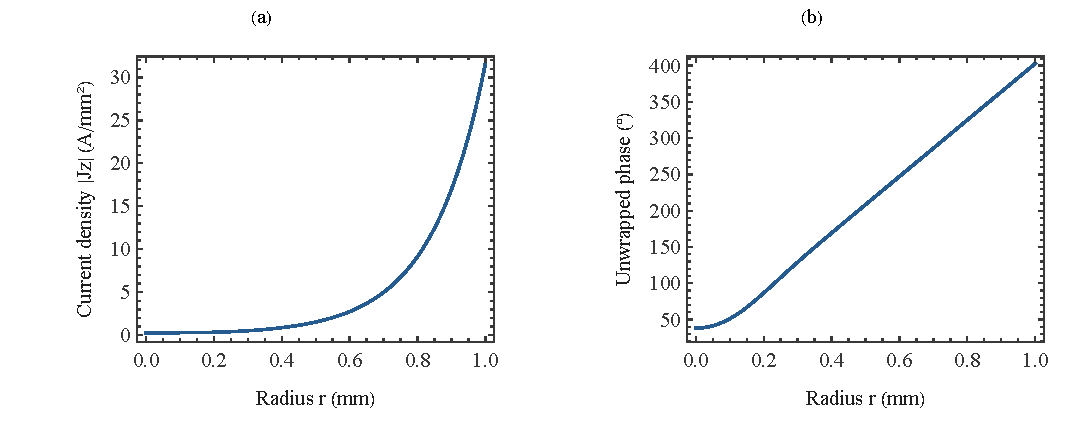
\includegraphics[width=\linewidth,height=.72\textheight,keepaspectratio]{../../assets/en/q1_profile.pdf}
\caption{Round-wire radial current magnitude and phase. The copper conductor has diameter 2 mm and carries 20 A RMS at 200 kHz. (a) RMS magnitude; (b) continuously displayed phase. Phase is displayed with a continuous radial lift, while magnitude retains RMS normalization. Radial samples come from preserved Bessel analytical data.}
\label{fig:q1_profile}
\end{figure}

% block-id: 03.figure.q1_cross_section
\hypertarget{03.figure.q1_cross_section}{}
\begin{figure}[!htbp]
\centering
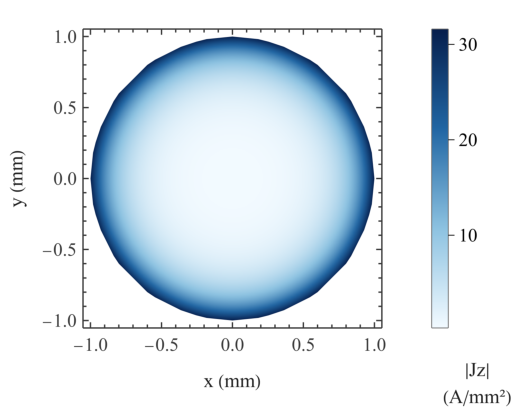
\includegraphics[width=\linewidth,height=.72\textheight,keepaspectratio]{../../assets/en/q1_cross_section.pdf}
\caption{Analytical round-wire cross-sectional magnitude. The copper conductor has diameter 2 mm and carries 20 A RMS at 200 kHz. The color scale represents axial RMS current density. Radial samples are linearly interpolated and mapped axisymmetrically. Coordinates are displayed in millimetres and current density in A/mm².}
\label{fig:q1_cross_section}
\end{figure}

% block-id: 03.figure.q1_fem_error
\hypertarget{03.figure.q1_fem_error}{}
\begin{figure}[!htbp]
\centering
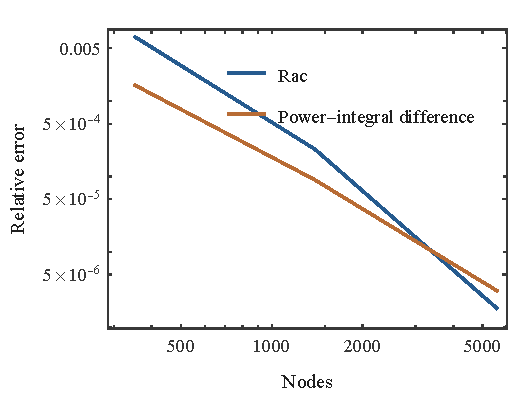
\includegraphics[width=\linewidth,height=.72\textheight,keepaspectratio]{../../assets/en/q1_fem_error.pdf}
\caption{Round-wire two-dimensional calibration errors. The copper conductor has diameter 2 mm and carries 20 A RMS at 200 kHz. Three grids and independent power integrals concern the same internal-field problem. Resistance is referenced to the internal Bessel solution of the same round wire. Power is evaluated by independent integration over the material region.}
\label{fig:q1_fem_error}
\end{figure}
